Supplementary material for chapter \ref{chap:rep} and its corresponding manuscript: {\bf Human copy number variants are enriched in regions of low mappability}.

%% Create counter for supp figs ("S1" etc)
\setcounter{figure}{0}
\renewcommand{\thefigure}{S\ref{chap:rep}.\arabic{figure}}
\setcounter{table}{0}
\renewcommand{\thetable}{S\ref{chap:rep}.\arabic{table}}

\section*{Supplementary Tables}


\begin{table}[htp]
  \centering
  \resizebox{\textwidth}{!}{
    \begin{tabular}{|c|r|r|r|l|c|c|}
      \hline
      Validated & Chr. & Start     & End       & Class        & Left PCR primer                & Right PCR primer               \\
      \hline
      V      & 3    & 6649794   & 6654897   & large CN 0   & CCTTAGTATTTCAGTGGTTTCTGTAGGTAT & ATAAATATCAGTGCTCAACTTGGACTT    \\
      V      & 5    & 127407030 & 127411341 & large CN 0   & TATTCATATTAACCTATCCTCACAGAAAGA & TTTTTAAGAGATTTGAACTAAAATTCCAC  \\
      V      & 3    & 5535139   & 5539535   & large CN 0   & TACTTTTTGAATTTGTAAATTTCCTTTGTA & GAAATCAGAAAATCAAGATCATACTGAAG  \\
      V      & 1    & 116229111 & 116233162 & large CN 0   & GTGTTACAGAATTAGTTTTACTGAGTGGTC & ATCTATAAAGAACTTTTTCCAAATAAACCA \\
      V      & 1    & 158961082 & 158966958 & large CN 1   & GTAGAATGAGCTGTGTTATGAGATGGT    & ATGACTTTCTATTGTTTGAAATGTAGTGAC \\
      V      & 15   & 26748887  & 26752614  & large CN 1   & CAATTTATCTATCAAGTTATTTCACGGTAG & AGTGAGATTTCATTTTAAGCTTGTCTTC   \\
      V      & 6    & 33937344  & 33942846  & large CN 1   & ACATTGTAGCCTGATGACCTTGTTC      & TGTGTTCTGAGGTTTACTTTATAATCTAGG \\
      V      & 12   & 82095501  & 82099389  & large CN 1   & ACCTATAACTAAGTGTAGCTGCTGTAACTG & TCAGTAAAAATGATTACTACAGTGGAAAAT \\
      V      & 5    & 8255604   & 8260914   & large CN 1   & TGAACATACATTCATACACACATAATACAA & TACATCACTGAACAAACCTCTATAGTCATA \\
      V      & 20   & 7398397   & 7403743   & large CN 1   & AATAAACATTCTCTATAAACCCTAAAATGG & CTTTGTACCATATTTCATAAACGTAGAGTC \\
      V      & 18   & 40053822  & 40057873  & large CN 1   & TAACTTTCTTTTCTAAAGCTTTTGGAGTAT & GTGAATTAAGATTCAATGTCTCTGCTAATA \\
      V      & 16   & 48904951  & 48906510  & small CN 0   & TCTTATTTATTTTGACAGTCCTTTACTCTG & AGATAATCAACTCTTTGTTTATTCTTTCAG \\
      V      & 2    & 241086647 & 241087801 & small CN 0   & ATCAACATTTAGCCAGTGTTGTCTTAG    & GTCTCTTGTGCTCTATCTTTGGCTT      \\
      V      & 13   & 110221621 & 110222631 & small CN 0   & ACCTCAGGAGAACTACTTCATACATTTCTA & GTATGAAAAACACTCATGGATATCATTTCT \\
      V      & 11   & 60571017  & 60572170  & small CN 0   & AATGTTGAAGTGTGTCTTTCTGTAATATCT & GTGTTTTGTGTCGCTATTTGTTTAGTA    \\
      V      & 5    & 166402295 & 166404219 & small CN 0   & TCACTTTATTCATAACATTTCAGTGTAGAG & GATCATATGCTTAAAATGCTAATGAGG    \\
      N     & 3    & 160126422 & 160127288 & small CN 1   & TAAGATACAAGAAATAGAGATAACACTGGG & TCTGAACACTTATTTTAAGAAAATGAAAAA \\
      N     & 17   & 10612674  & 10613775  & small CN 1   & AATTTAGCAGTCTCTTACATTTCTTCTACC & TCTCTTCTATAAAAATAAATGGCTAAAAGC \\
      V      & 10   & 70253713  & 70255155  & small CN 1   & AATAAAATCAAAGGTGATATTACTGACAGA & ATATACTCTTTTAACTTTTGACCATTTTGG \\
      V      & 8    & 53700635  & 53702050  & small CN 1   & TAAGGAAAATTTAGTATAGTCTGGACCTGT & ATGGAAATATATCTCTGATGGGTGAC     \\
      % N     & 6    & 26636844  & 26637539  & low coverage & GTACATAGATTCTCACCCACAATTAAATC  & CTTCTTCAACATCAGACAGTACACATT    \\
      % N     & 13   & 78236245  & 78238105  & low coverage & GTCAGTCTGGTTCTTTTCTGTCAAG      & ACTTTAGTAAAATTGTTATTTAGTCCCAGG \\
      % V      & 1    & 248546279 & 248548008 & low coverage & CTATCTTTCTTACCATTTAATATCTGCCTT & AGACTTCATTTAGGAAAGTGAGAAATACAC \\
      \hline
    \end{tabular}
  }
  \caption[Experimental validation results.]{{\bf Experimental validation results.} {\small Location of the validated (V) and non-validated (N) CNVs for different classes. The last two columns show the primer sequences used for PCR amplification.}}
  \label{tab:pcr}
\end{table}

\begin{table}[htp]
  \centering
  \resizebox{\textwidth}{!}{
    \begin{tabular}{|r|r|r|l|r|r|l|l|l|}
      \hline
      Chr. & Start & End & CN & PCR product size & PCR product size when deletion & Validated & Gel & Sanger Sequencing\\
      \hline
      14 & 40098378 & 40100213 & 0 & 2586 & 751 & Yes & Different bands & Yes: confirmed\\
      \hline
      5 & 85559864 & 85564846 & 1.05 & 5690 & 708 & Yes & Different bands & Yes: confirmed\\
      \hline
      6 & 14299746 & 14299801 & 0.79 & 755 & 700 & Yes & Double bands & No\\
      \hline
      7 & 153000055 & 153000246 & 1.76 & 1137 & 946 & Yes & Double bands & Yes: confirmed\\
      \hline
      4 & 96401034 & 96401460 & 1.13 & 745 & 319 & Yes & Double bands & No\\
      \hline
      16 & 34230052 & 34230512 & 1 & 1139 & 679 & Yes & Double bands & No\\
      \hline
      16 & 8688137 & 8689592 & 1.02 & 2121 & 666 & Yes & Double bands & Yes: confirmed\\
      \hline
      2 & 12018994 & 12022932 & 1.02 & 4291 & 353 & Yes & Double bands & Yes: confirmed\\
      \hline
      3 & 121051576 & 121060845 & 1.14 & 9485 & 216 & Yes & Double bands & No\\
      \hline
      3 & 54433855 & 54433912 & 0 & 952 & 895 & Yes & One band & Yes: insertion\\
      \hline
      2 & 151031059 & 151038246 & 1.11 & 7485 & 298 & Yes & Small band only & No\\
      \hline
      9 & 45462450 & 45462522 & 1.1 & 530 & 458 & No & One band & No\\
      \hline
      7 & 63233184 & 63233261 & 1.33 & 390 & 313 & No & One band & Yes: nothing\\
      \hline
      9 & 106371251 & 106371330 & 1.28 & 484 & 405 & No & One band & No\\
      \hline
      16 & 20466400 & 20466487 & 1.27 & 393 & 306 & No & One band & No\\
      \hline
      5 & 85559864 & 85564842 & 0.78 & 5690 & 712 & No & One band & No\\
      \hline
      10 & 65703860 & 65708900 & 1.64 & 5430 & 390 & No & One band & No\\
      \hline
      7 & 159117395 & 159122761 & 1.09 & 5909 & 543 & No & One band & No\\
      \hline
      2 & 83066824 & 83068234 & 0.57 & 2097 & 687 & NA & No amplification & No\\
      \hline
      13 & 35996202 & 35996254 & 1.13 & 546 & 494 & NA & Non-specific & No\\
      \hline
      4 & 159799983 & 159801372 & 1.03 & 2313 & 924 & NA & Non-specific & Yes: not clear\\
      \hline
      7 & 52963172 & 52964911 & 1.48 & 2316 & 577 & NA & Non-specific & No\\
      \hline
      10 & 69323932 & 69326507 & 1.62 & 2795 & 220 & NA & Non-specific & Yes: not clear\\
      \hline
      6 & 58618198 & 58624080 & 1.04 & 6518 & 636 & NA & Non-specific & No\\
      \hline
    \end{tabular}
  }
  \caption[Experimental validation in low-coverage regions.]{{\bf Experimental validation in low-coverage regions.} {\small The result of the PCR validation was either concordant with {\sf PopSV} call (Yes), discordant (No) or inconclusive (NA). In some cases, Sanger sequencing was performed. The {\it CN} column is the estimated copy-number of the deleted allele.}}
  \label{tab:pcr2}
\end{table}

\begin{table}[htp]
  \centering
  \resizebox{.6\textwidth}{!}{
    \begin{tabular}{|r|r|r|}
      \multicolumn{3}{l}{{\bf Homozygous deletion}} \\
      \hline
       deletion support & reference support & number of calls \\
      \hline
      0   & 0   & 11     \\
      0   & 1   & 1      \\
      1   & 0   & 1      \\
      2   & 0   & 12     \\
      \hline
      \multicolumn{3}{l}{{\bf Heterozygous deletion}} \\
      \hline
       deletion support & reference support & number of calls \\
      \hline
      0   & 0   & 18     \\
      0   & 1   & 10     \\
      0   & 2   & 7      \\
      1   & 0   & 6      \\
      1   & 1   & 4      \\
      1   & 2   & 4      \\
      2   & 0   & 10     \\
      2   & 1   & 3      \\
      \hline
    \end{tabular}
  }
  \caption[Investigating low-mappability deletion calls with two CEPH12878 assemblies.]{{\bf Investigating low-mappability deletion calls with two CEPH12878 assemblies.} {\small The first two columns represent the number of assemblies (0, 1 or 2) supporting the deleted allele or the reference allele. The third column shows the number of {\sf PopSV} calls in each category.}}
  \label{tab:cephAss}
\end{table}

\begin{table}[htp]
  \centering
  \resizebox{\textwidth}{!}{
    \begin{tabular}{|l|r|rrr|r|r|rr|}
      \hline
      \multirow{2}{*}{CNV catalog} & \multirow{2}{*}{Samples} & \multicolumn{3}{c|}{Variants} & \multirow{2}{*}{Avg Size (Kbp)} & Proportion & \multicolumn{2}{c|}{Affected genome (Mbp)} \\
      
                                          &       & Total  & \multicolumn{2}{c|}{Per sample} &           & $<$3 Kbp & Total & Per sample    \\
      \hline
                                          &       &        & {\it WG}                        & {\it ELC} &          &       &        &      \\
      1000GP                              & 2,504 & 41,979 & 1,024.44                        & 2.22      & 6.00     & 0.68  & 580.03 & 6.14 \\
      {\it ~~deletion}                    &       & 36,102 & 975.32                          & 2.21      & 4.67     & 0.72  & 342.97 & 4.56 \\
      {\it ~~duplication}                 &       & 8,503  & 48.26                           & 0.00      & 32.54    & 0.00  & 331.48 & 1.57 \\
      \hline                                
      GoNL                                & 750   & 9,592  & 1,048.14                        & 0.63      & 2.93     & 0.81  & 65.30  & 3.07 \\
      {\it ~~deletion}                    &       & 9,009  & 1,013.35                        & 0.63      & 2.36     & 0.82  & 34.79  & 2.39 \\
      {\it ~~duplication}                 &       & 528    & 21.11                           & 0.00      & 29.19    & 0.15  & 30.63  & 0.62 \\
      \hline                                
      Handsaker 2015 ({\sf Genome STRiP}) & 847   & 8,657  & 212.03                          & 1.88      & 27.80    & 0.00  & 196.57 & 5.89 \\
      {\it ~~deletion}                    &       & 5,961  & 145.78                          & 0.56      & 21.64    & 0.00  & 108.03 & 3.15 \\
      {\it ~~duplication}                 &       & 3,469  & 66.26                           & 1.32      & 41.35    & 0.00  & 118.28 & 2.74 \\
      \hline                                
      Chiang 2017 ({\sf Genome STRiP})    & 148   & 7,932  & 828.49                          & 9.23      & 6.35     & 0.42  & 73.20  & 5.26 \\
      \hline
    \end{tabular}
  }
    \caption[Properties of events in public CNV catalogs]{{\bf Properties of events in public CNV catalogs.} {\small Deletions, duplications and CNVs from four public catalogs. Variants with high frequency ($>80\%$), variants on the chromosome X, and variants smaller than 300 bp were removed in order to compare with {\sf PopSV}'s numbers (Table \ref{tab:res}). WG: whole genome; ELC: extremely low-coverage regions. The {\it Total} number of variants is the total number after collapsing recurrent variants. {\it Affected genome} represents the amount of the reference genome that overlaps at least one CNV.}}
  \label{tab:1kgp}
\end{table}


\begin{table}[htp]
  \centering
  \resizebox{.8\textwidth}{!}{
    \begin{tabular}{|l|l|l|l|l|}
      \cline{1-2}\cline{4-5}              
      Novel region          & OMIM gene && Novel region           & OMIM gene \\
      \cline{1-2}\cline{4-5}              
      1:25730001-25736000   & RHCE      && 9:136418001-136420000  & ADAMTSL2  \\
      \cline{1-2}\cline{4-5}              
      1:161640001-161645000 & FCGR2B    && 10:64130001-64135000   & ZNF365    \\
      \cline{1-2}\cline{4-5}              
      1:207705001-207715000 & CR1       && 10:101595001-101600000 & ABCC2     \\
      \cline{4-5}                         
      1:207725001-207745000 & CR1       && 10:135380001-135383500 & SYCE1     \\
      \cline{1-2}\cline{4-5}                                       
      5:68845001-68886000   & OCLN      && 11:320001-325000       & IFITM3    \\
      \cline{1-2}\cline{4-5}                                      
      5:69360001-69365000   & SMN2      && 12:52683001-52685000   & KRT81     \\
      \cline{4-5}                         
      5:69373001-69374000   & SMN2      && 12:52696001-52696500   & KRT86     \\
      \cline{1-2}\cline{4-5}                                       
      5:70165001-70222000   & SMN1      && 15:32454001-32460000   & CHRNA7    \\
      5:70242001-70242500   & SMN1      && 15:32464001-32464500   & CHRNA7    \\
      \cline{4-5}                         
      5:70246501-70258000   & SMN1      && 15:43902501-43903000   & STRC      \\
      \cline{1-2}
      6:29905001-29910000   & HLA-A     && 15:43910001-43910500   & STRC      \\
      \cline{1-2}\cline{4-5}                                       
      6:31960001-31975000   & C4A       && 16:21760001-21765000   & OTOA      \\
      \cline{1-2}\cline{4-5}                                       
      6:31995001-31995500   & C4B       && 17:34504001-34545000   & CCL3L3    \\
      \cline{1-2}\cline{4-5}                                       
      6:32522001-32560000   & HLA-DRB1  && 19:11535001-11540000   & CCDC151   \\
      \cline{1-2}\cline{4-5}                                       
      6:32590001-32602000   & HLA-DQA1  && 19:41340001-41350000   & CYP2A6    \\
      \cline{1-2}\cline{4-5}                                       
      6:32628501-32629000   & HLA-DQB1  && 22:18660001-18765000   & USP18     \\
      \cline{4-5}                                       
      6:32630001-32634000   & HLA-DQB1  && 22:18904501-18905500   & PRODH     \\
      \cline{1-2}
      7:39052001-39055500   & POU6F2    && 22:18909001-18909500   & PRODH     \\
      \cline{1-2}\cline{4-5}                                       
      7:74195001-74200000   & NCF1      &       \multicolumn{3}{c}{}        \\
      \cline{1-2}
    \end{tabular}
  }
  \caption[OMIM genes overlapping novel CNV regions of low-mappability]{{\bf OMIM genes overlapping novel CNV regions of low-mappability} {\small Novel CNV regions are polymorphic in more than 1\% of the individuals across the three cohorts but absent from the 1000GP SV catalog\cite{Sudmant2015a}. OMIM genes are genes associated with a disease or phenotype in the OMIM Morbid Map (Online Mendelian Inheritance in Man; \url{http://omim.org/}).}}
  \label{tab:omimgenes}
\end{table}


\clearpage

\section*{Supplementary Figures}

\begin{figure}[htp]
  \centering
  \begin{subfigure}[b]{.48\textwidth}
    \includegraphics[width=\linewidth,page=2]{figures/wgs-map-coverage-cohorts.pdf}
    \caption{}
    \label{fig:mapcov}
  \end{subfigure}
  \begin{subfigure}[b]{.48\textwidth}
    \includegraphics[width=\linewidth,page=3]{figures/wgs-map-coverage-cohorts.pdf}
    \caption{}
    \label{fig:meancov}
  \end{subfigure}

  \begin{subfigure}[b]{.48\textwidth}
    \includegraphics[width=\linewidth,page=7]{figures/wgs-map-coverage-cohorts.pdf}
    \caption{}
    \label{fig:meancohort}
  \end{subfigure}
  \begin{subfigure}[b]{.48\textwidth}
    \includegraphics[width=\linewidth,page=8]{figures/wgs-map-coverage-cohorts.pdf}
    \caption{}
    \label{fig:sdcohort}
  \end{subfigure}

  \caption[Coverage, mappability and population-based measures]{{\bf Coverage, mappability and population-based measures.} {\small a-b) Read coverage in a sample (y-axis) versus mappability (a) or the inter-sample average coverage (b). c-d) Inter-sample mean (c) and standard deviation (d) were fitted against the mappability in each cohort separately. The tiles represent all cohorts pooled together.}}
\end{figure}

\begin{figure}[htp]
  \centering
  \begin{subfigure}[b]{.48\textwidth}
    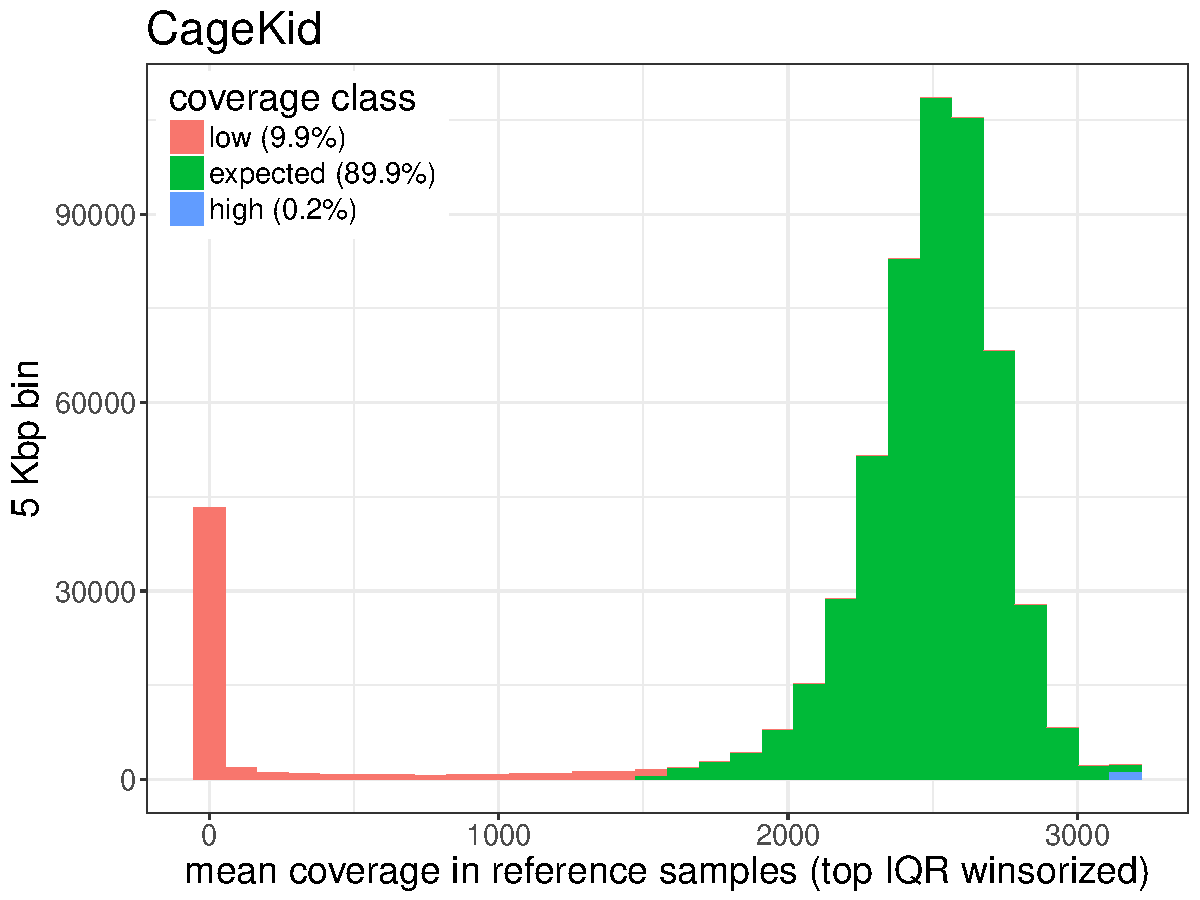
\includegraphics[width=\linewidth,page=1]{figures/wgs-coverage-tracks-cagekid-gonl.pdf}
    \caption{}
  \end{subfigure}
  \begin{subfigure}[b]{.48\textwidth}
    \includegraphics[width=\linewidth,page=3]{figures/wgs-coverage-tracks-cagekid-gonl.pdf}
    \caption{}
  \end{subfigure}

  \caption[Average coverage in reference samples in the CageKid and GoNL datasets.]{{\bf Average coverage in reference samples in the CageKid (a) and GoNL (b) datasets.}}
  \label{fig:covclass2}
\end{figure}

\begin{figure}[htp]
  \includegraphics[width=\linewidth,page=5]{figures/replication-twins.pdf}
  \caption[Rand index between pedigree and CNV-based dendogram in low-coverage regions.]{{\bf Rand index between the pedigree information and the dendogram from CNV calls in low-coverage regions.} {\small The dendogram for CNV-based clustering was cut at different levels (x-axis) and the groups compared to the pedigree (family-level) with the Rand index (y-axis). For each method, the line highlights the best performance across three linkage criteria.}}
  \label{fig:randindex}
\end{figure}

\begin{figure}[htp]
  \includegraphics[width=\linewidth,page=2]{figures/replication-cagekid.pdf}
  \caption[{\sf PopSV}'s performance in low-mappability regions in CageKid dataset.]{{\bf {\sf PopSV}'s performance in low-mappability regions in CageKid dataset.} {\small Proportion and number of calls replicated in the paired tumor. The point shows the median value per sample, the error bars the 95\% confidence interval.}}
  \label{fig:replication:cagekid}
\end{figure}

\begin{figure}[htp]
  \includegraphics[width=\linewidth,page=2]{figures/PopSV-NA12878-assembly-lowMap.pdf}
  \caption[Distance to assembly gaps and supporting evidence from long-read sequencing in CEPH12878.]{{\bf Distance to assembly gaps and supporting evidence from long-read sequencing in CEPH12878.} {\small Deletions in low-mappability regions were grouped by their supporting evidence (y-axis and colors). {\it assemblies}: deletion observed in at least one of the two public assemblies. {\it PB-SV}: overlap with a structural variant called from the PacBio reads\cite{Pendleton2015}. {\it PB-reads}: deletion observed in the local assembly or consensus of the PacBio reads. Variants with no support are represented by the white boxplot.}}
  \label{fig:cephGap}
\end{figure}

\begin{figure}[htp]
  \centering
  \includegraphics[width=\linewidth,page=3]{figures/PopSV-catalog-overview.pdf}
  \caption[Overlap between {\sf PopSV} catalog and calls from Pendleton et al..]{{\bf Overlap between {\sf PopSV} catalog and calls from Pendleton et al..} {\small Recurrent calls were collapsed in each catalog (i.e {\sf PopSV} and the 1000 Genomes Project (1000GP)). The proportion of the collapsed calls overlapping calls from \citet{Pendleton2015} was computed. The fold-enrichment is produced by drawing control regions with similar size distribution as Pendleton's calls. {\it low-map}: calls in low-mappability regions; {\it ext. low-map}: calls in extremely low-mappability regions.}}
  \label{fig:pendcat}
\end{figure}

\begin{figure}[htp]
  \centering
  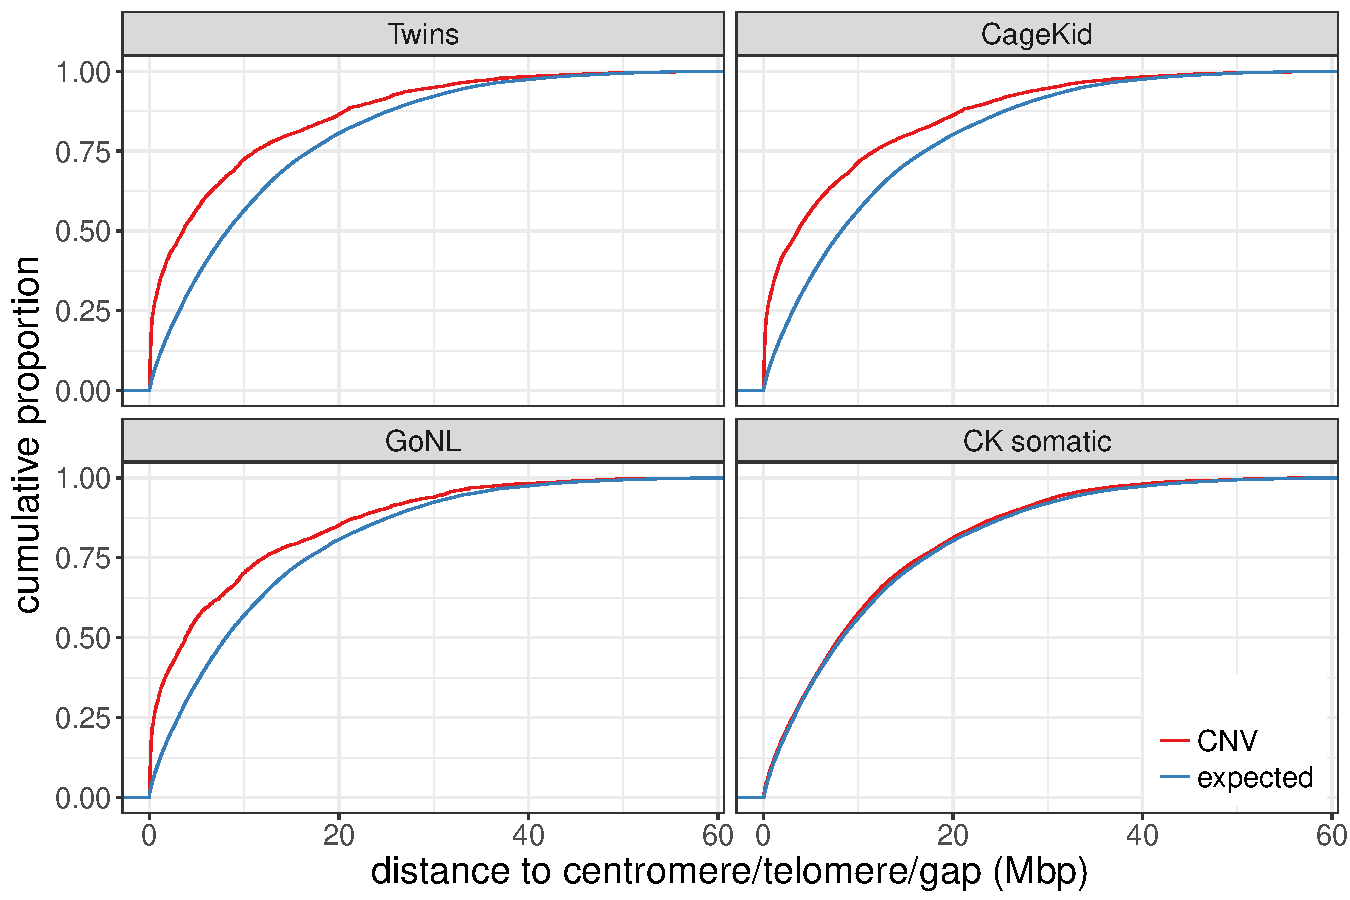
\includegraphics[width=\textwidth,page=1]{figures/PopSV-repeatEnr.pdf}
  \caption[Distance to a centromere, telomere or assembly gap.]{{\bf Distance to a centromere, telomere or assembly gap.} {\small The y-axis represents the cumulative proportion of the affected genome. The {\it expected} curve is computed from uniformly distributed genomic regions with matched size.}}
  \label{fig:ctgDist}
\end{figure}

\begin{figure}[htp]
  \centering
  \begin{subfigure}{.9\textwidth}
    \includegraphics[width=\textwidth,page=2]{figures/PopSV-repeatEnr-long.pdf}
    \caption{}
    \label{fig:repCont}
  \end{subfigure}
  
  \begin{subfigure}{.48\textwidth}
    \includegraphics[width=\textwidth,page=4]{figures/PopSV-repeatEnr.pdf}
    \caption{}
    \label{fig:repSat}
  \end{subfigure}
  \begin{subfigure}{.48\textwidth}
    \includegraphics[width=\textwidth,page=6]{figures/PopSV-repeatEnr.pdf}
    \caption{}
    \label{fig:repSR}
  \end{subfigure}
  \caption[CNVs enrichment after controlling for segmental duplication overlap and distance to CTG.]{{\bf CNVs enrichment after controlling for segmental duplication overlap and distance to CTG.} {\small Enrichment of CNVs in a) different genomic features, b) satellite families and c) simple repeats in the different cohorts (colors). Bars show the median fold enrichment across samples compared to control regions. The star represents significant enrichment from the logistic regression.}}
\end{figure}

\begin{figure}[htp]
  \centering
  \begin{subfigure}{.48\textwidth}
    \includegraphics[width=\textwidth,page=5]{figures/PopSV-repeatEnr.pdf}
    \caption{Satellites}
  \end{subfigure}
  \begin{subfigure}{.48\textwidth}
    \includegraphics[width=\textwidth,page=7]{figures/PopSV-repeatEnr.pdf}
    \caption{Simple repeats}
  \end{subfigure}

  \begin{subfigure}{.48\textwidth}
    \includegraphics[width=\textwidth,page=9]{figures/PopSV-repeatEnr.pdf}
    \caption{Transposable elements}
  \end{subfigure}
  \caption[Overlap between CNVs and repeats.]{{\bf Overlap between CNVs and repeats.} {\small The histograms represent the proportion of the CNV region that overlaps a) a satellite, b) a simple repeat or c) a transposable element, when they do overlap. The {\it expected} distribution is computed from the control regions used for the enrichment analysis.}}
  \label{fig:repeatOl}
\end{figure}

\begin{figure}[htp]
  \centering
  \begin{subfigure}{.7\textwidth}
    \includegraphics[width=\textwidth,page=4]{figures/example-L1PA-NAHR.pdf}
    \caption{}
  \end{subfigure}
  
  \begin{subfigure}{.7\textwidth}
    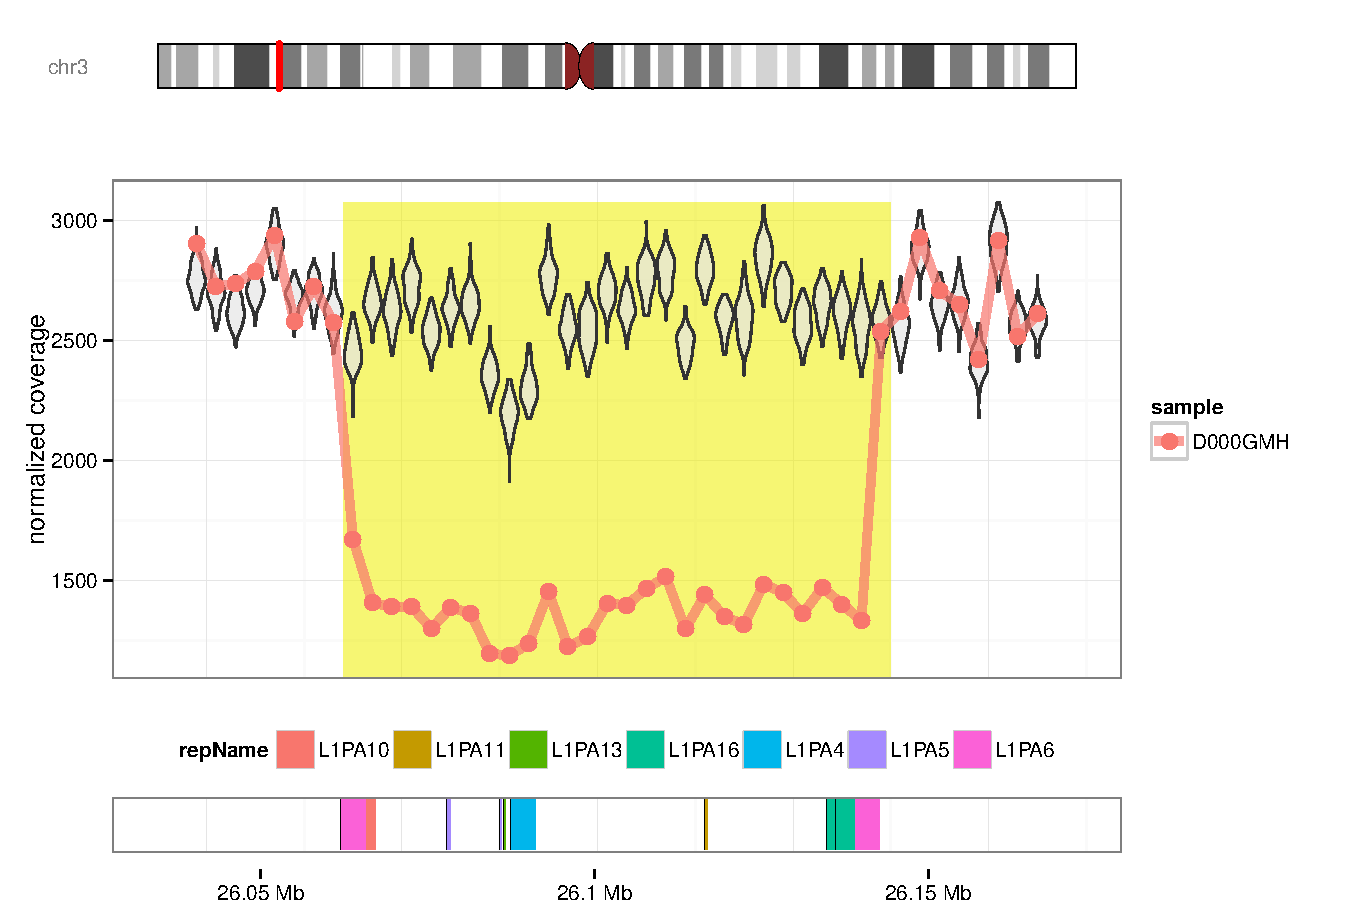
\includegraphics[width=\textwidth,page=1]{figures/example-L1PA-NAHR.pdf}
    \caption{}
  \end{subfigure}
  \caption[Polymorphism likely caused by non-homologous allelic recombination between L1PA repeats.]{{\bf Polymorphism likely caused by non-homologous allelic recombination between L1PA repeats.} {\small Examples of CNV likely caused by non-allelic homologous recombination between two L1PA3 repeats (a) or L1PA6 (b). The line and points represent the coverage of one sample with a duplication (a) or a deletion (b), highlighted in yellow; the violin plots represent the distribution of the coverage in the reference samples. }}
  \label{fig:l1pa}
\end{figure}


\begin{figure}[htp]
  \centering
  \includegraphics[width=\textwidth,page=6]{figures/PopSV-catalog-overview.pdf}
  \caption[Novel CNV regions and CNVs in other public catalogs]{{\bf Novel CNV regions and CNVs in other public catalogs.} {\small Cumulative proportion of the 3,455 novel regions (y-axis) that overlap CNVs in different public CNV catalogs (colour) depending on their frequency in the public catalog (x-axis). The labels highlight the proportion of novel regions that don't overlap any CNV in the corresponding public catalog. Novel regions were defined as overlapping a CNV in more than 1\% of the individuals but absent from the 1000GP catalog.}}
  \label{fig:novelcatfreq}
\end{figure}





\clearpage

\section*{Supplementary Information}
\label{sec:suppmat:reppopsv}

\section*{Data}
\label{sec:data}

\paragraph{Twin study}
All patients gave informed consent in written form to participate in the Quebec Study of Newborn Twins\cite{Boivin2013}. Ethic boards from the Centre de Recherche du CHUM, from the Université Laval and from the Montreal Neurological Institute approved this study. Sequencing was done on an Illumina HiSeq 2500 (paired-end mode, fragment length ~300 bp). The reads were aligned using a modified version of the Burrows-Wheeler Aligner ({\sf bwa} version 0.6.2-r126-tpx with threading enabled). The options were \verb!'bwa aln -t 12 -q 5'! and \verb!'bwa sampe -t 12'!.
The aligned reads are available on the European Nucleotide Archive under \href{https://www.ebi.ac.uk/ena/data/view/PRJEB8308}{ENA PRJEB8308}.
The 45 samples had an average sequencing depth of 40x (minimum 34x / maximum 57x).

\paragraph{Renal cell carcinoma}
WGS data from renal cell carcinoma is presented in details in the CageKid paper\cite{Scelo2014}.
In short, 95 pairs of normal/tumor tissues were sequenced using GAIIx and HiSeq2000 instruments.
Paired-end reads of size 100 bp totaled an average sequencing depth of 54x (minimum 26x / maximum 164x).
Reads were trimmed with {\sf FASTX-Toolkit} and mapped per lane with {\sf BWA} backtrack to the GRCh37 reference genome.
{\sf Picard} was used to adjust pairs coordinates, flag duplicates and merged lane.
Finally, realignment was done with {\sf GATK}.
Raw sequence data have been deposited in the European Genome-phenome Archive, under the accession code \href{https://www.ebi.ac.uk/ega/studies/EGAS00001000083}{EGAS00001000083}.

\paragraph{Genome of the Netherlands}
WGS data from the GoNL project is described in details in \citet{Francioli2014}. This data have been derived from different sample collections:
\begin{itemize}
\item The LifeLines Cohort Study (\url{http://www.lifelines.nl/}), supported by the Netherlands Organization of Scientific Research (NWO, grant 175.010.2007.006), the Dutch government's Economic Structure Enhancing Fund (FES), the Ministry of Economic Affairs, the Ministry of Education, Culture and Science, the Ministry for Health, Welfare and Sports, the Northern Netherlands Collaboration of Provinces (SNN), the Province of Groningen, the University Medical Center Groningen, the University of Groningen, the Dutch Kidney Foundation and Dutch Diabetes Research Foundation.
\item The EMC Ergo Study (\url{http://www.ergo-onderzoek.nl/wp/}).
\item The LUMC Longevity Study, supported by the Innovation-Oriented Research Program on Genomics (SenterNovem IGE01014 and IGE05007), the Centre for Medical Systems Biology and the National Institute for Healthy Ageing (Grant 05040202 and 05060810).
\item VU Netherlands Twin Register (\url{http://www.tweelingenregister.org/}).
\end{itemize}

In short, samples were sequenced on an Illumina HiSeq 2000 instrument (91-bp paired-end reads, 500-bp insert size).
We downloaded the aligned read sequences (BAM) for the 500 parents in the data set.
We further performed indel realignment using {\sf GATK} 3.2.2, adjusted pairs coordinates with {\sf Samtools} 0.1.19, marked duplicates with {\sf Picard} 1.118, and performed base recalibration ({\sf GATK} 3.2.2).
The average sequencing depth was 14x (minimum 9x / maximum 59x).

\paragraph{Genomic annotations} Gencode annotation (V19) was directly downloaded from the consortium FTP server at \url{ftp://ftp.sanger.ac.uk/pub/gencode/Gencode_human/release_19/gencode.v19.annotation.gtf.gz}.
Other genomic annotations were downloaded from the UCSC database\cite{Rosenbloom2015} server at \url{http://hgdownload.soe.ucsc.edu/goldenPath/hg19/database}.
The file names of the corresponding annotations are
\label{sec:genodata}

\medskip

\begin{tabular}{|l|l|}
  \hline
  Mappability                          & \verb!wgEncodeCrgMapabilityAlign100mer.bw! \\
  Cytogenetic bands                    & \verb!cytoBandIdeo.txt.gz!                 \\
  Centromere, telomere, assembly gap   & \verb!gap.txt.gz!                          \\
  Segmental duplication                & \verb!genomicSuperDups.txt.gz!             \\
  Simple repeat / Short Tandem Repeats & \verb!simpleRepeat.txt.gz!                 \\
  RepeatMasker                         & \verb!rmsk.txt.gz!                         \\
  \hline
\end{tabular}

\section*{Read count across the genome}

The genome was fragmented in non-overlapping bins of fixed size.
The number of properly mapped reads was used as a coverage measure, defined as read pairs with correct orientation and insert size, and a mapping quality of 30 (Phred score) or more.
In each sample, GC bias was corrected by fitting a LOESS model between the bin's coverage and the bin's GC content.
For each bin, the correction factor was computed as the mean coverage across all the bins divided by the predicted coverage from the LOESS model and the GC content of the bin.
We used a bin size of 5 Kbp for most of the analysis.
When specified, we used a smaller bin size of 500 bp.

\section*{RD and mappability estimates}

To investigate the bias in RD we used the read counts in 5 Kbp bins.
Bins with extremely high coverage were identified and removed when deviating from the median coverage by more than 5 standard deviation.
First the coverage of the 45 samples from the Twin study were combined and quantile normalized.
At that point the different samples had the same global coverage distribution and no bins with extreme coverage or GC bias.

The mappability track\cite{Derrien2012} was downloaded from UCSC\cite{Rosenbloom2015} \\(\verb!wgEncodeCrgMapabilityAlign100mer.bw!) and the average mappability was computed for each bin.
One sample was randomly selected and we compared its coverage with the mappability estimates.
We then computed the mean and standard deviation of the coverage in each bin across the other samples and compared it with the sample coverage.
We also compared the inter-sample average with the mappability estimates.

To compute Z-scores that integrates the observed coverage variation we used two approaches.
The first modeled the coverage metrics (average or standard deviation) using the mappability estimates and computed a Z-score from the predicted coverage and global standard deviation.
A generalized additive model was fitted using a cubic regression spline on the mappability estimates ({\sf mgcv} R package).
In the second approach, Z-scores were computed using the inter-sample average and standard deviation.
The normality of these two Z-score distributions were compared in term of excess kurtosis and skewness.
For the kurtosis and skewness computation, we removed outlier Z-scores with an absolute value greater than 10. These bins could be regions of CNV and would bias the estimates.
The Z-score distributions were also compared in bins from 10 different mappability intervals.

We repeated this analysis pooling 45 samples from each of the three datasets.
After quantile normalization, the inter-sample coverage mean and standard deviation were computed separately in each cohort and compared with the mappability estimates.

\section*{CNV detection with {\sf PopSV}}

\paragraph{Binning the genome}
We ran two separate analysis on the three datasets.
Bin sizes of 5 Kbp and 500 bp were used on the Twin study and renal cell carcinoma.
Because of its lower sequencing depth, the 500 bp run on GoNL gave only partial results.
More precisely, we observed a truncated distribution of the copy-number estimates, with most of the 1 and 3 copy number variants missing.
It means that at this resolution many one-copy variation cannot be differentiated from background noise.
For this reason we ran GoNL analysis using 2 Kbp and 5 Kbp bins.

\paragraph{Constructing the set of reference samples}
In each dataset we choose the reference samples as follows: in the renal cancer dataset from the normal samples, in the Twin study from all the samples, in GoNL from a subset of 200 samples (see below).
For each dataset, a Principal Component Analysis (PCA) was performed across samples on the counts normalized globally (median/variance adjusted).
The resulting first two principal components are used to verify the homogeneity of the reference samples.
Although our three datasets showed different levels of homogeneity, we didn't need to exclude samples or split the analysis.
The effect of weak outlier samples was either corrected by the normalization step or integrated in the population-view.

In GoNL, we decided to use only 200 of the 500 samples as reference.
They were selected to span a maximum of the space defined by the principal components.
In contrast to random selection, this ensures that weak outliers are included in the final set of reference samples, hence maximizing the technical variation integrated in the population-view.

Moreover, the principal components were used to select one control sample from the final set of reference samples.
This sample is used in the normalization step as a baseline to normalize other samples against.
We picked the sample closest to the centroid of the reference samples in the Principal Component space.

\paragraph{CNV calling}
After targeted normalization the coverage in each sample is compared to the coverage in the reference samples.
A Z-score is computed and translated into a P-value that is then corrected for multiple testing.
Consecutive bins with significant excess or lack of reads are merged and returned as potential duplication or deletion.
Copy number estimates are derived from the coverage across the bin and the average coverage across the reference samples.
However, it is important to note that the definition of a variant is different from other methods.
Here a variant is defined by the major allele in the population rather than the reference genome state.
Most of the genome is in a diploid state compared to the reference genome and sufficiently covered by sequencing reads that the copy number state can be correctly estimated by {\sf PopSV}'s population-based approach.
However, highly polymorphic variants are called relative to the major allele in the population and additional efforts are required to assess the copy number state.
Variants in extremely low-mappability regions are also difficult to fully characterize and might be caused by rare insertion in the reference genome or complex alleles.
Nonetheless, {\sf PopSV} can efficiently detect the presence of CNV in any situation.
More details are available in the method paper\cite{Monlong2018}.

\paragraph{Coverage tracks}
For each run, we constructed coverage tracks based on the average coverage in the reference samples.
Bins where the reference samples had, on average, the expected coverage were classified as {\it expected coverage}.
Bins with a coverage lower than 4 standard deviation from the median were classified as {\it low-mappability}(or {\it low coverage}).
To ensure robustness, the standard deviation was derived from the Median Absolute Deviation.
We use regions with low coverage to define {\it low-mappability regions}, as the low coverage is a result of the lower mappability of a region.
Because the standard deviation is used, the number of regions classified as {\it low-mappability} is lower in datasets with more RD variance.

Eventually, we also defined {\it extremely low coverage} region which have an average coverage below 100.
This sub-class of {\it low coverage} region was used in a few analyses to highlight the most challenging regions.

Regions were annotated with the overlap with protein-coding genes and segmental duplications (see \nameref{sec:genodata}), and the distance to the nearest centromere, telomere or assembly gap.
Finally, we computed the number of protein-coding genes overlapping at least one low-coverage region.

\section*{Validation and benchmark}

\paragraph{Running {\sf FREEC}, {\sf CNVnator}, {\sf cn.MOPS} and {\sf LUMPY}}
{\sf FREEC}\cite{Boeva2011} segments the RD values of a sample using a LASSO-based algorithm.
It was run on each sample separately, starting from the BAM file, using the same bin sizes as for {\sf PopSV}.
{\sf FREEC} internally corrects the RD for GC and mappability bias.
In order to compare its performance in low-mappability region, the minimum {\it ``telocentromeric''} distance was set to 0.
The remaining parameters were set to default.
Of note an additional run with slightly looser parameter (\verb!breakPointThreshold=0.6!) was performed to get a larger set of calls used in some parts of the {\it in silico} validation analysis to deal with borderline significant calls.

{\sf CNVnator}\cite{Abyzov2011} uses a mean-shift technique inspired from image processing.
It was run on each sample separately, starting from the BAM file, using the same bin sizes as for {\sf PopSV}.
{\sf CNVnator} also corrects internally for GC bias and we used default parameters.
For the analysis using higher confidence calls, we used calls with either 'eval1' or 'eval2' lower than $10^{-5}$ (instead of the default 0.05).

{\sf cn.MOPS}\cite{Klambauer2012} considers simultaneously several samples and detects copy number variation using a Poisson model and a Bayesian approach.
It was run on the same GC-corrected bin counts used for {\sf PopSV}.
All the samples are analyzed jointly.
Of note an additional run with slightly looser parameter (\verb!upperThreshold=0.32! and \verb!lowerThreshold=-0.42!) was performed to get a larger set of calls used in some parts of the {\it in silico} validation analysis to deal with borderline significant calls.

{\sf LUMPY}\cite{Layer2012} which uses an orthogonal mapping signal: the insert size, orientation and split mapping of paired reads.
The discordant reads were extracted from the BAMs using the recommended commands.
Split-reads were obtained by running {\sf YAHA}\cite{Faust2012} with default parameters.
All the CNVs (deletions and duplications) larger than 300 bp were kept for the upcoming analysis.
\verb!BND! variants with both ends more than 300 bp apart in the same chromosome were also included as they could be CNVs lacking support to characterize their type properly.
Calls with 5 or more supporting reads were considered high-confidence.

\paragraph{Clustering samples from the Twin study}
A distance between two samples A and B was defined as : $1 - 2\frac{|R_A \cap R_B|}{|R_A| + |R_B|}$ where $R_A$ represents the regions called in sample A, $R_A \cap R_B$ the regions called in both A and B, and $|R|$ the cumulative size of the regions.
Hence, the similarity between two samples is represented by the amount of sequence found in both divided by the average amount of sequence called.
This distance is used for hierarchical clustering of the samples in the Twin dataset.
The clustering was performed using only calls in regions with extremely low coverage (reference average $\le$100 reads).
Different linkage criteria ({\it average}, {\it complete} and {\it Ward}) were used for the exploration.
In our dendograms we used the {\it average} linkage criterion.
The concordance between the clustering and the pedigree was estimated by the Rand index, grouping the samples per family.
For each method and linkage criteria, the Rand index was computed for every possible dendogram cut ({\it x}-axis in Figure \ref{fig:randindex}).

\section*{Experimental validation}
Experimental validation was performed on samples from the Twin study.
In a first validation batch, variants were randomly selected among both one-copy and two-copy deletions.
We selected both small ($\sim700$ bp) and large ($\sim4$ Kbp) variants in each class.
%%In addition, 3 deletions in low-mappability regions were also randomly selected and included.
The coverage at base pair resolution was visually inspected for each deletion and, when possible, the breakpoints were fine-tuned.
PCR primers were designed to target the whole deleted region.
We randomly selected 20 variants out of the variants for which we managed to design PCR primers.
We then performed long-range PCR followed by gel electrophoresis.
PCR was performed using 50 ng of DNA and the Phusion High-Fidelity DNA Polymerase from Thermo Fisher Scientific: 95 $^{\circ}$C 5 minutes followed by 35 cycles (95 $^{\circ}$C 30 seconds, 64 $^{\circ}$C 30 seconds, 72 $^{\circ}$C 45 seconds) and 72 $^{\circ}$C 10 minutes.
Either a 1\% or 1.8\% aragose gel was used, depending on the expected size of the amplified fragments.
We used a 1 Kb Plus DNA Ladder from Thermo Fisher Scientific.

The presence of a deletion was tested by comparing the size of the amplified fragment in affected and control samples.
If the affected sample showed a lower band than a control with a predicted 2 copies, the deletion was considered validated.
On the other hand if affected sample and controls had one similar band, the deletion was considered non-validated.
Of note, the validation rate might be under-estimated because visual prediction of the breakpoint is not always accurate.

We then randomly selected deletions overlapping low-mappability regions and detected in 6 samples or fewer.
We chose to test rare variants because they are likely enriched in false-positives.
Hence, this batch of validation represents the most challenging regions to call and validate, and enriched in false-positives.
Here we couldn't use the base-pair coverage to fine-tune the breakpoints because the low-mappability blurs any clear signal.
Instead, we retrieved the reads (and their pairs) mapping to the region and assembled them.
With this approach we could sometimes get a better breakpoint resolution and design PCR primers that would amplify the deleted region.
In addition to gel electrophoresis, the amplified DNA of some regions was sequenced using Sanger sequencing.
We randomly selected 17 variants out of the variants for which we managed to design PCR primers.

\section*{Analysis of CEPH12878}

\paragraph{Whole-Genome Sequencing data}
High coverage PCR-free Illumina WGS data for 30 samples, including CEPH12878, was downloaded from the 1000 Genomes Project\cite{Sudmant2015a}.
The ENA accession number is \href{http://www.ebi.ac.uk/ena/data/view/PRJNA260854}{PRJNA260854}.
The files are also available on the FTP server at \url{http://ftp.1000genomes.ebi.ac.uk/vol1/ftp/release/20130502/supporting/high_coverage_alignments/20141118_high_coverage.alignment.index}.
Although the sequencing depth is similar to the other datasets (average $\sim$53X), the reads are 250 bp long so the average number of reads per region is lower.
Because of the lower read coverage and sample size the CNV calls will be of slightly lower quality.
Nonetheless, {\sf PopSV} was run using 5 Kbp bins and all the samples as reference.
Using the same coverage track as before we then selected all deletions in CEPH12878 and overlapping low-mappability regions (at least 90\% of the call).
We then looked for support in public assemblies, SV catalogs and reads from long-read sequencing technologies.

\paragraph{Comparison with assemblies}
We downloaded the genome assembly produced from short reads, Pacbio and BioNano reads\cite{Pendleton2015} from \url{ftp://ftp.ncbi.nlm.nih.gov/genomes/all/GCA/001/013/985/GCA_001013985.1_ASM101398v1/GCA_001013985.1_ASM101398v1_genomic.fna.gz}.
We also downloaded a second assembly that was used 10X Genomics linked reads instead of the Pacbio reads\cite{Mostovoy2016}.
It is available at \url{http://kwoklab.ucsf.edu/resources/nmeth_201604_NA12878_hybrid_assembly.fasta.gz}

For each selected variant, we retrieved the two 50 Kbp flanking sequences in the reference genome and aligned them against the public assemblies with {\sf BLAST}\cite{Camacho2009}.
The output was parsed to identify regions with two flanks aligning in at least 1 Kbp of a contig.
MUMmer plots\cite{Kurtz2004} between the reference sequence and the contigs were visually inspected.
The assembly supported {\sf PopSV} calls when a deletion was visible in the expected region (between the flanks).
The assembly supported the reference genome sequence when a contig crosses the variant without clear structural variant.

\paragraph{SV calls from a long-read sequencing study}
We downloaded the SV calls from the Pacbio reads and assembled contigs in \citet{Pendleton2015}.
The VCF file is publicly available at \url{ftp://ftp-trace.ncbi.nlm.nih.gov/giab/ftp/data/NA12878/NA12878_PacBio_MtSinai/NA12878.sorted.vcf.gz}.
We overlapped {\sf PopSV} calls with deletions from this SV catalogs.
Because we used 5 Kbp bins for {\sf PopSV}, at least 1 Kbp of a {\sf PopSV} calls needed to overlap a deletion from \citet{Pendleton2015} to be considered as sufficient support.
Of note, the distribution of the overlap tended to be either null or higher than 1 Kbp supporting this choice.

\paragraph{Local assembly of Pacbio reads}
Corrected Pacbio reads from citet{Pendleton2015} were downloaded from \url{ftp://ftp-trace.ncbi.nlm.nih.gov/giab/ftp/data/NA12878/NA12878_PacBio_MtSinai/corrected_reads_gt4kb.fasta}.
Each read was split in 200 bp fragments and mapped to the human reference genome (version hg19).
From this mapping information we selected full Pacbio reads with at least one 200 bp mapping within a region of interest (with 30 Kbp flanks).
For each region, the reads were mapped to the reference sequence with exonerate and we kept reads with partial mapping as they may support a SV.
These reads were then assembled using {\sf Canu}\cite{Koren2017}.
A consensus sequence was also derived for reads clustered by alignment breakpoint and the {\sf clustalo}\cite{Sievers2011} software.
The assembled contigs and consensus were mapped to the reference genome to identify a potential breakpoint.
The two regions flanking the alignment breakpoint and the sequence spanning the breakpoint were mapped to the entire genome.
We used the results of this genome-wide mapping to select the best candidates: assembled sequence whose flanks align uniquely to the region of interest and with reduced alignment quality for the ``middle'' sequence that spanned the breakpoint.
Candidate contig/consensus were further visualized with MUMmer plots\cite{Kurtz2004}.
The assembly supported {\sf PopSV} calls when a deletion was visible in the expected region (between the flanks).


\section*{Genomic patterns of CNVs}

\paragraph{Merging calls from two different bin sizes}
Small bins gives better resolution for smaller variants.
Large bins gives better sensitivity.
For this reason we merged the calls from the 500 bp bin and 5 Kbp bin runs.
Variant supported by both sets of calls were merged into one.
To decide which set to use for the breakpoints and other information (e.g. copy number estimate), the proportion of overlap was used.
If call(s) using small bins overlapped more than a third of a call from the large bin run, it was considered fully recovered by the small bin call which was then used to define breakpoints and other information.
If not, the large bin run was considered more appropriate to define the final breakpoints and additional information.
Calls unique to each run were simply added to the final set of calls.
For the Twin dataset and the renal cancer dataset, calls from the 500 bp and 5Kbp runs were merged.
For the GoNL dataset, calls from the 2 Kbp and 5Kbp runs were merged.

\paragraph{Computing global estimates of copy number variation}
In Table \ref{tab:res}, a call in extremely low coverage region is overlapped at more than 90\% by the {\it extremely low coverage} track.
To compute the total number of calls, we collapsed calls with an overlap higher than 50\%.
The amount of sequence affected in a genome was computed by merging all the variants in the cohort and counting the number of affected bases in this reference genome.
After the merging step, each base of the genome either overlapped a merged variant or not.
Each affected base was counted only once, even if it overlapped CNVs in several samples or with large copy number differences.

\paragraph{Comparison with public CNV catalogs}
The SV catalog from \citet{Sudmant2015a} was downloaded from \url{http://ftp.1000genomes.ebi.ac.uk/vol1/ftp/phase3/integrated_sv_map/ALL.wgs.mergedSV.v8.20130502.svs.genotypes.vcf.gz}.
The CNV catalog from \citet{Handsaker2015} was downloaded from \url{http://www.broadinstitute.org/\%7Ehandsake/mcnv_data/bulk/1000G_phase1_cnv_genotypes_phased_25Jul2014.genotypes.vcf.gz}
For the CNV catalog from \citet{Chiang2017}, we downloaded \verb!GTEx_Analysis_2016-10-24_WholeGenomeSeq_147Indiv_SV_sites.vcf.gz! from the GTEx Data Portal at \url{https://www.gtexportal.org/home/datasets} (data release v6).
The CNV catalog from \citet{Francioli2014} was downloaded from \url{https://molgenis26.target.rug.nl/downloads/gonl_public/variants/release6.1/20161013_GoNL_AF_genotyped_SVs.vcf.gz}.
We retrieved the set of autosomal deletion, duplication and CNVs.
When comparing the global estimates of CNV with {\sf PopSV}, we removed deletions smaller than 300 bp as well as variants with high frequency ($>80\%$).
This remaining SVs represent CNVs that could in theory be detected by {\sf PopSV}'s approach.
Using this sub-set, we derived the number of variants, number of variants smaller than 3 Kbp, number of variants in {\it extremely low coverage} regions, and amount of genome affected.
These number are computed exactly as the one presented in Table \ref{tab:res} for {\sf PopSV}'s results.

\paragraph{CNV frequency comparison}
The frequency at which a region is affected by a CNV is computed using calls from the 620 unrelated samples.
The copy-number change is not taken into account in the computation and the frequency is derived for all the nucleotide that overlaps at least one CNV.
Using each catalog we computed, for each base in the genome, the proportion of individuals with a CNV.
This frequency measure facilitates the comparison of catalogs with different methods and resolution.
We represented the distribution as a cumulative proportion distribution in Figure \ref{fig:freq1kgp}.
The graphs read as ``how much of the total affected genome is called in at more than X\% of the population''.
The frequency distribution was computed separately for deletions and duplications (and {\it CNV} in the 1000 Genomes Project catalog).
Of note, the 1000 Genomes Project was down-sampled to 640 random individuals in order to give comparable frequency curves.

\paragraph{Comparison with CNV catalogs from long-read studies}
First, the SV catalog from \citet{Chaisson2014} was downloaded from \\
\url{http://eichlerlab.gs.washington.edu/publications/chm1-structural-variation/}.
Recurrent calls were collapsed in both {\sf PopSV} and the 1000 Genomes Project catalogs.
{\sf PopSV}'s catalog corresponded to all germline calls in the Twin study, renal cancer dataset and GoNL.
The 1000 Genomes Project catalog contained all the deletions, duplications and CNVs, no matter the size or frequency.
The analysis was also performed separately on deletions, duplications, low-mappability regions and extremely low-mappability regions.
For each comparison, we randomly selected control regions with sizes and overlap with assembly gaps similar to the SVs in \citet{Chaisson2014} (see \nameref{sec:controlreg}).
A logistic regression tested the enrichment of CNVs in the Chaisson catalog versus the control regions.
The regression was performed on 50 different sampling of the control regions for each comparison.
The 50 samplings are represented by the boxplot in Figure \ref{fig:chaisson}.
We compared the estimates from the logistic regression.
They represent the log odds ratio of a CNV overlapping the catalog from Chaisson.
The same analysis was performed using the SV catalog from \citet{Pendleton2015} downloaded from \url{ftp://ftp-trace.ncbi.nlm.nih.gov/giab/ftp/data/NA12878/NA12878_PacBio_MtSinai/NA12878.sorted.vcf.gz}.

\paragraph{Distance to centromere, telomere and assembly gaps}
The centromeres, telomeres and assembly gaps (CTGs) are annotated in the {\sf gap} track from UCSC\cite{Rosenbloom2015}.
However, some chromosomes were missing telomere annotations.
We defined them as the 10 Kbp region at the ends of chromosomes derived from the cytogenetic bands track.

The distance from each variant to the nearest CTG was computed and represented as a cumulative proportion, i.e. the proportion of variants located at a distance $d$ or closer to a CTG.

Because this distribution changes with the size of the variants, we sampled random regions in the genome with similar sizes and computed the same distance distribution (see \nameref{sec:controlreg}).
Thanks to this null distribution we were able to see if variants were located closer/further to CTG than expected by chance.

\paragraph{Selecting control regions}
\label{sec:controlreg}
In several analyses we compared the CNVs with control regions.
The control regions have the same size distribution as the regions they are derived from (e.g. CNV, annotation).
In some analysis we further controlled for the overlap with specific genomic features.
For example, we controlled for the overlap with CTGs to avoid selecting control regions in assembly gaps where no CNV or annotation is available.
Controlling for the overlap with regions flanking CTGs, we could simply control for the distance to CTGs.
We also used this approach to control for the overlap with segmental duplications and investigate patterns independent from this repeat class.

To select control regions, thousands of bases were first randomly chosen in the genome.
The distance between each base and the genomic features was then computed.
At this point, simulating a region of a specific size and with specific overlap profile can be done by randomly choosing as center one of the bases that fit the profile :

\begin{equation}
  \label{eq:controlreg}
  \left\{b,  \forall~feature~f, O_f(d_f^b - \frac{S_r}{2}) < 0\right\}  
\end{equation}

\noindent with $O_f$ equals 1 if the original region overlaps with feature $f$, -1 if not; $d_f^b$ is the distance between base $b$ and feature $f$; and $S_r$ is the size of the original region.

For each input region, a control region was selected as described and had by construction the exact same size and overlap profile.

\paragraph{Enrichment in genomic features}
We tested different genomic features, starting with: genes, exons, low-mappability regions, segmental duplications, satellites, simple repeats and transposable elements.
The different satellite families, frequent simple repeat motives, transposable element families were also tested.
We overlapped each genomic feature with CNVs and control regions.
We then computed the fold change in proportion of regions overlapping a feature, in CNV versus control regions.
A pseudo count was added when computing this ratio:

\begin{equation}
  \label{eq:foldenr}
  \mbox{Fold enrichment} = \frac{\frac{|CNV \cap Feature|+1}{N+1}}{\frac{|Control \cap Feature|+1}{N+1}} = \frac{|CNV \cap Feature|+1}{|Control \cap Feature|+1} 
%  \stackrel{Fold}{Enrichment} = \frac{|CNV \cap Feature|+1}{N+1} \Big/ \frac{|Control \cap Feature|+1}{N+1} = \frac{|CNV \cap Feature|+1}{|Control \cap Feature|+1} 
\end{equation}
  
\noindent where $N$ is the number of CNVs (and control regions).

The fold enrichments were computed separately for each sample using control regions that fitted perfectly the profile of the variants in the sample.
To assess the significance of the enrichment, a logistic regression was performed using CNV and control regions.
The model to test one feature in one sample was:

\begin{equation}
  \label{eq:lr}
  \log \left( \frac{P(\mbox{feature overlap})}{P(\mbox{no overlap})} \right) = \beta_0 + \beta_{CNV} \cdot CNV
\end{equation}


\noindent with $ CNV = \left\{ \begin{array}{ll} 0 & \mbox{if control region} \\ 1 & \mbox{if CNV} \\ \end{array} \right. $

\medskip

To control for the enrichment in segmental duplication we used control regions with similar overlap profile (see \nameref{sec:controlreg}).
We also added a variable representing the overlap with segmental duplication in the model:

\begin{equation}
  \label{eq:lrsd}
  \log \left( \frac{P(\mbox{feature overlap})}{P(\mbox{no overlap})} \right) = \beta_0 + \beta_{CNV} \cdot CNV + \beta_{SD} \cdot SD
\end{equation}


\noindent with $ SD = \left\{ \begin{array}{ll} 0 & \mbox{if no SD overlap} \\ 1 & \mbox{if SD overlap} \\ \end{array} \right. $

For each feature and cohort we computed the median P-value.
When numerous tests were performed (e.g. satellite families, simple repeat motives, transposable element families or sub-families), the P-values were first corrected for multiple testing using Benjamini-Hochberg procedure.

Finally, we computed the proportion of the region overlapped by the different features (satellites, simple repeats and transposable elements).
We compared CNV regions and control regions.

\paragraph{Somatic variant definition}
Somatic variants were defined as variant in a tumor samples with low overlap with variant in the paired normal sample.
In CageKid data, overlapping tumor variant with the ones from the paired normal showed almost only two peaks, at 0 and 100\% overlap.
A tumor variant was defined as somatic if it overlapped less than 10\% of any variant in the paired normal.



%%% Local Variables:
%%% mode: latex
%%% TeX-master: "../main"
%%% End:
